% ====================================================================
%+
% SECTION:
%    supernovacosmology.tex
%
% CHAPTER:
%    cosmology.tex
%
% ELEVATOR PITCH:
%    SNIa cosmology, approach to evaluating dependence of science on cadence
%
% COMMENTS:
%
%
% BUGS:
%
%
% AUTHORS:
%    Phil Marshall (@drphilmarshall)  - put your name and GitHub username here!
%-
% ====================================================================

\section{Supernova Cosmology and Physics}
\def\secname{supernovae}\label{sec:\secname}
% \label{sec:cosmology, supernovae, classification, lenstimedelays, deepdrillingfields }

\noindent{\it Jeonghee Rho, Michelle Lochner, Rahul Biswas, Seth Digel} % (Writing team)

% This individual section will need to describe the particular
% discoveries and measurements that are being targeted in this section's
% science case. It will be helpful to think of a ``science case" as a
% ``science project" that the authors {\it actually plan to do}. Then,
% the sections can follow the tried and tested format of an observing
% proposal: a brief description of the investigation, with references,
% followed by a technical feasibility piece. This latter part will need
% to be quantified using the MAF framework, via a set of metrics that
% need to be computed for any given observing strategy to quantify its
% impact on the described science case. Ideally, these metrics would be
% combined in a well-motivated figure of merit. The section can conclude
% with a discussion of any risks that have been identified, and how
% these could be mitigated.

This section is concerned with the detection and characterization of supernovae (SNe)
over time with LSST and their various scientific applications.
The most important
application is the use of supernovae type Ia (SNIa) and potentially some core-collapse SN (like type IIP) to trace the recent expansion history of the universe,
and confront models of the physics driving the late time accelerated expansion
of the universe. 

This objective of SN cosmology follows (at least for SNIa) results from several
highly successful surveys; improvement in knowledge of cosmology could come from
substantially larger numbers of well-characterized SNe.
This
goal is not directly tied to the unprecedentedly large survey area of LSST.  
However, we shall argue that in practice, even this
goal would benefit from the spatial scale offered by the WFD
component of the LSST survey. 

On the other hand, the WFD aspect will make the LSST survey potentially the 
first to scan the very large area of the entire Southern sky for SNe. 
SNe that are detected and well characterized by LSST will
probe the isotropy of the universe.  Peculiar velocities of 
SNe will probe the growth of structure.  In addition, this large sample
will enable further
sharpening of our understanding of the properties of the SN population 
of different types. 
This last point is extremely important for SN cosmology goals:  The success of SNIa cosmology has always been based on the empirical model that intrinsic peak brightnesses are related to the certain observable characteristics of SNe. 
%While the spatial locations of the SNe are not important
The 
WFD SNIa sample will dramatically increase the size of the sample 
available to train such an empirical model, as well understand the probability of deviations and scatter from this model. Aside from issues like calibration 
which need to be addressed differently, a larger sample of such well measured SNe is probably the only way to address `systematics' due to deviations from the empirical
model. The anticipated sample can be thought of as consisting of two 
components:  the low-redshift sample which is more likely to be complete, and the higher-redshift sample that will be able to constrain evolution. 
% --------------------------------------------------------------------

\subsection{Target measurements and discoveries}
\label{sec:keyword:targets}

% Describe the discoveries and measurements you want to make.

SNe of different types are visible over time scales of about a few 
weeks (e.g., type Ia) to nearly a year (type IIP).  During the full ten-year
 survey, LSST will scan the entire southern sky repeatedly
 with a WFD cadence, and certain specific locations
of the sky called the Deep Drilling Fields (DDF) with special enhanced cadence. 

This spatio-temporal window should contain millions \todo{RB}{remember to check} of SNe, that will have apparent magnitudes brighter than the single exposure limiting magnitude of LSST.  However, the actual
 sequence of observations by LSST, defined by the series of field pointings as a
 function of time in filter bands (along with weather conditions), will
 determine the extent to which each SN can be detected and
 characterized well.  Characterization of the SNe is at the core of a
 number of science programs that use them as bright, abundant objects with empirically determined intrinsic brightnesses. For LSST, this goal entails (a) detection of SNe, (b) photometric typing of SNe, (c) estimating photometric redshifts of SNe (or identifying host galaxies 
 and obtaining their redshifts from photometry or follow-up spectroscopy),
(d) estimation of intrinsic brightnesses of the SNe, and finally (e) use of these data in addressing our science goals of cosmological inference, etc.
The efficacy of photometric typing, redshifts and estimation of intrinsic brightnesses are all
dependent on the amount of information available in the observed light curves of SNe. While these steps are not necessarily independent, it is useful to think of the requirements on some of these steps separately; it is not unlikely  that combinations of some of the steps would still be affected by similar requirements. 

{\emph{Our first objective is to detect such SNe}}, by which we mean
selecting SNe from among the transient sources detected by LSST.
% classify them as SNe (as opposed to an AGN, or an asteroid). 
In brief, this process 
consists of defining a set of image subtractions between a high-resolution
`template` image of a sky section, and a set of single exposures at
different times (usually of lower resolution) of the same region, after 
accounting for the different resolutions of images, and alignments. These sets of image subtractions associated
 with a single object will be used to detect the object as a transient and then
classify the transient as an SN. Clearly, detecting an SN depends on the number of such images recorded per object, the different filters used for those images, and the signal-to-noise ratios of the images. %One might expect that 
The efficiency of this step may be summarized as a threshold on the joint properties 
of an astrophysical candidate (apparent brightness, light curve characteristics, background) as well as observing conditions (astronomical seeing, etc.).  

{\emph{Our second objective is to photometrically classify different kinds of SNe.}} 
%{\bfseries Photometric SN classification}\\
Previously, only spectroscopically typed SNe have been used for cosmology. Photometric 
typing from light curves alone has only been used to select candidates for spectroscopic 
follow-up (see, e.g., \citet{Sako2008}). However, LSST will simply find far too many 
candidates for even a significant fraction of them to be followed up spectroscopically. In order to avoid 
discarding the majority of the SN dataset, we need to use techniques capable of 
determining cosmological parameters from a potentially contaminated photometric SN dataset.

Several techniques have been proposed recently to solve this problem. One 
approach involves applying stringent cuts to the photometric dataset to obtain a nearly pure sample 
of SNIa\citep{Bernstein2012,Campbell2013} and running the standard SNIa cosmology analysis 
with this sample. Another approach, BEAMS \citep{Kunz2007,Newling2011,Hlozek2012,Knights2013}, 
makes use of an entire dataset, coping with contamination by using a mixture model for the 
likelihood, thus allowing for multiple populations. Whatever the technique ultimately used for 
cosmological analysis, it will rely on accurate initial classifications of SN type and 
unbiased estimates for the probability of each type.

Current state-of-the-art photometric classification techniques rely on fitting empirically 
determined templates of SNe to light curves \citep{Jha2007,Guy2007,Sako2011}. However in 
recent years, new approaches have been developed in response to the 2010 `Supernova 
Photometric Classification Challenge' \citep{Kessler2010a}. Many of these use novel light curve 
parameterization and employ machine learning algorithms to perform the classification (see \citet{Kessler2010b} and references therein).

While many of these methods have been tested on standard sets of simulated data and (in some cases) 
on SDSS data, which technique (if any) is superior in all situations is unclear. For 
example, some techniques are dependent on the availability of reliable redshift information. 
%, while others  are less reliant on it. 
Some techniques may be more robust to non-representative datasets [Not sure what this means] than 
others, and how the techniques will respond to changes in cadence, filter sets, signal-to-noise, 
etc., is unclear.  

With this in mind, we propose the use of a multifaceted classification system which employs 
several different methods for extracting features from the light curves (e.g., fitting parametric 
functions or templates) and several different classification algorithms. This system is highly 
modular, allowing new approaches for direct comparison with existing  techniques to be added easily. This also allows direct analysis of different observing strategies, without requiring 
an initial choice of classification technique. 


{\emph{Our third objective is to characterize SNe in terms of empirical
    light curve models.}}

The ultimate goal of using SNe (type SNIa or SNIIP) for cosmology requires estimating the intrinsic brightnesses of the SN. The
first (and sometimes only, depending on the light curve model) step is
fitting the calibrated fluxes to a light curve model with a set of parameters.
According to the ansatz used in SN cosmology, the intrinsic brightness of
 SNe is largely determined by the parameters of the light curve model; 
 hence the uncertainties on the inferred parameters largely determine the
 uncertainties on the inferred peak intrinsic brightness or distance moduli of the SNe.

% Now, describe their response to the observing strategy. Qualitatively,
% how will the science project be affected by the observing schedule and
% conditions? 

% In broad terms, how would we expect the observing strategy
% to be optimized for this science?





% --------------------------------------------------------------------

\subsection{Metrics}
\label{sec:keyword:metrics}

Quantifying the response via MAF metrics: definition of the metrics,
and any derived overall figure of merit.
\label{sec:keyword:metrics}

\begin{center}
\begin{tabular}{| p{5cm} |p{10cm} |p{2cm}}
\hline Metric & Description & Status\\
\hline
SN discovery I  &  Identify the number of LSST data points and quality required & \\
SN light curve quality & Generate SN light curves using OpSim output of baseline Cadence &\\
SN classification & Classify identified SNe into SN Ia, II, Ib, and Ic & \\
SN light curve II & Generate SN light curves with different redshift (0.1-1) &\\
SN discovery II &  Estimate the number of SN discovery as a function of redshift & \\
\hline \end{tabular}
 \end{center}


\emph{To be added: discussion of the ROC curve as a useful metric for photometric supernova 
classification}


\begin{figure*}[!hb]
    \begin{minipage}[b]{\linewidth}
        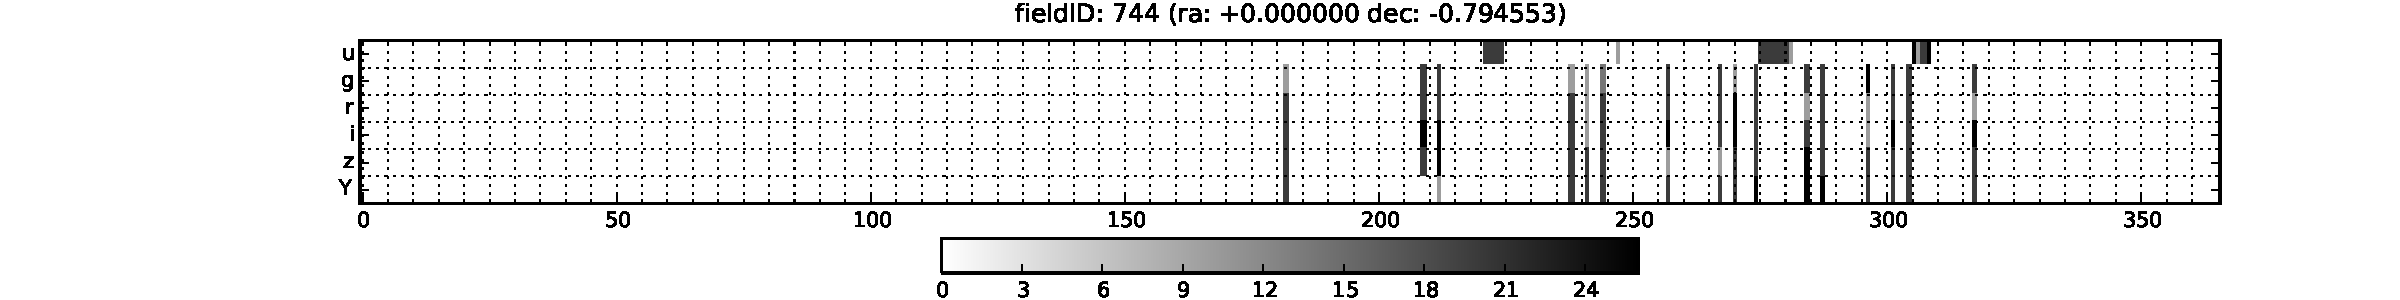
\includegraphics[width=\textwidth]{figs/supernova/fig_firstSeason_0}
        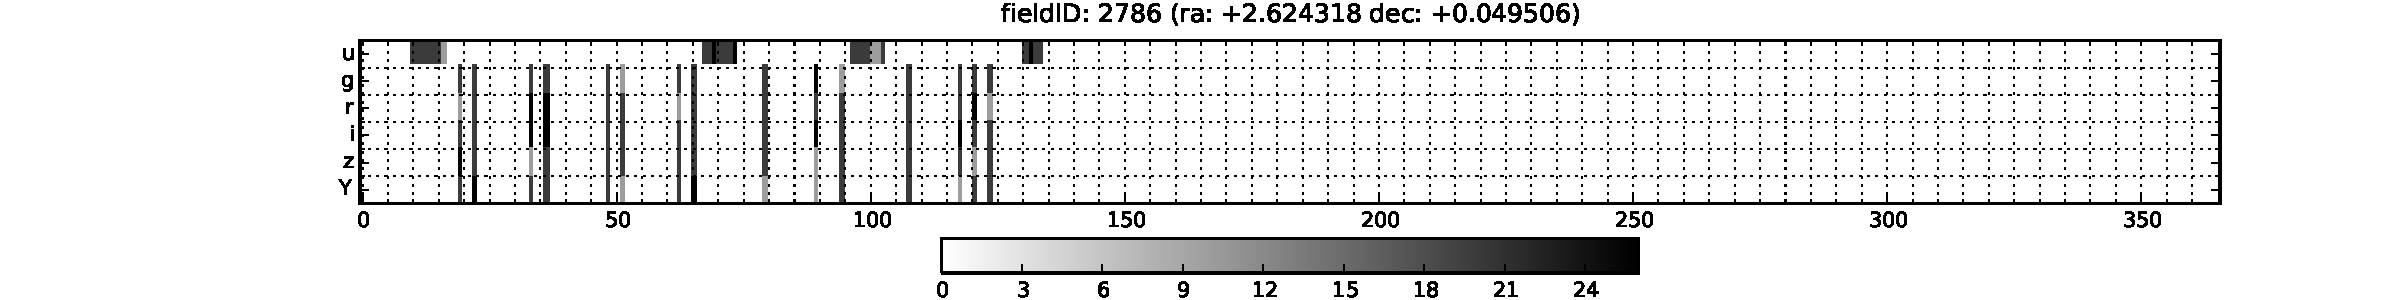
\includegraphics[width=\textwidth]{figs/supernova/fig_firstSeason_1}
        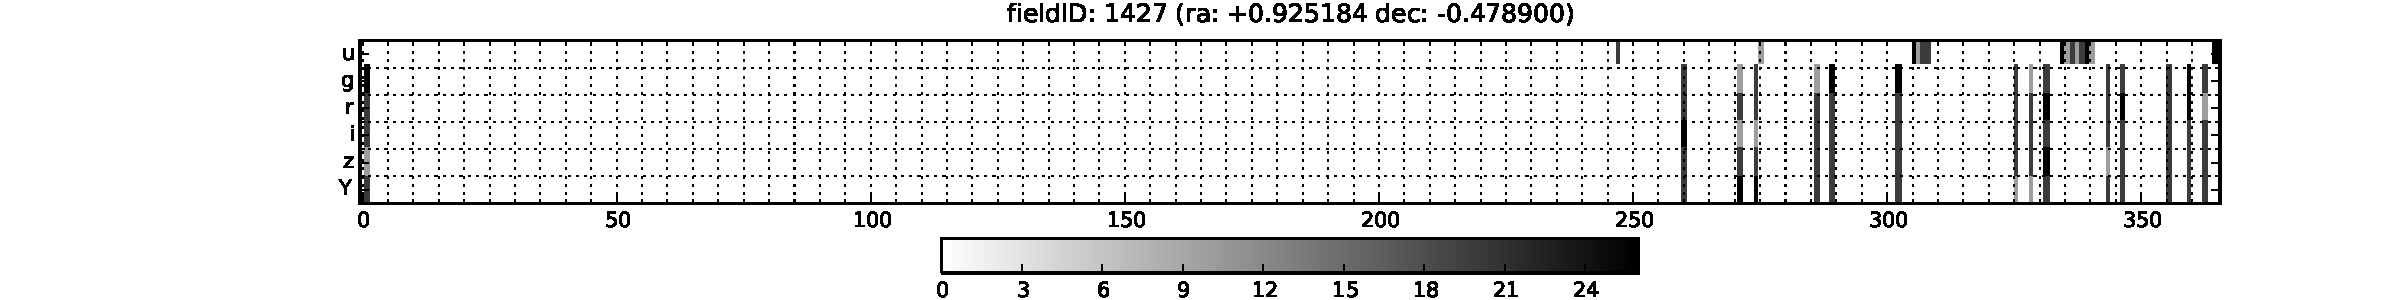
\includegraphics[width=\textwidth]{figs/supernova/fig_firstSeason_2}
        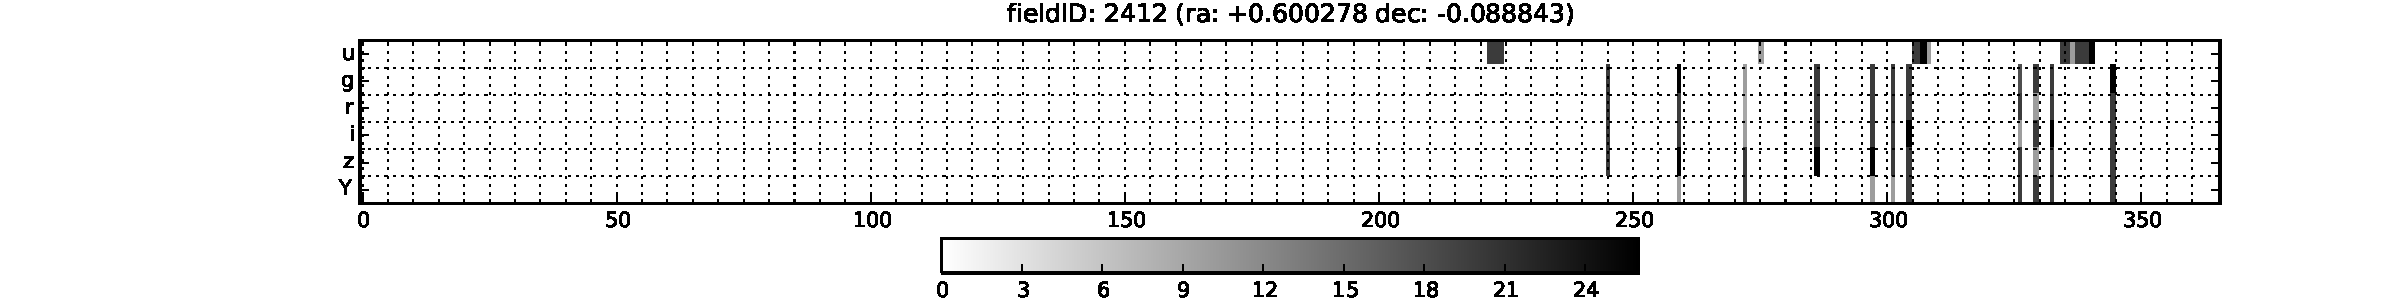
\includegraphics[width=\textwidth]{figs/supernova/fig_firstSeason_3}
        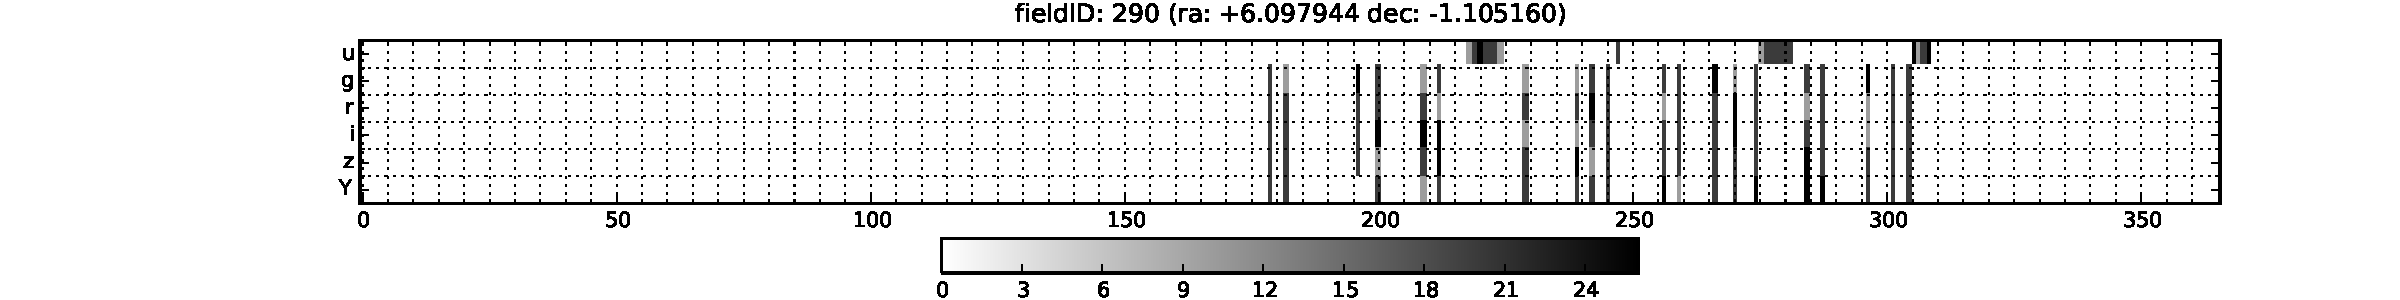
\includegraphics[width=\textwidth]{figs/supernova/fig_firstSeason_4}
    \end{minipage}
\label{fig:opsimSummary}
\caption{Include 1) an example of Type Ia Light Curve, 2) an example of Type II, 3) the number of SNR as a function of
redshift}
\end{figure*}


% --------------------------------------------------------------------

\subsection{OpsSim Analysis}
\label{sec:keyword:analysis}

{\bf Motivation and description:}

As noted above the scientific goal of characterizing SNe is to a large extent
dependent on how well the light curves of individual SNe are sampled in
time and filters. To study this, we re-index the OpsSim output on spatial
locations rather than use the temporal index. There are different methods (which will be merged), and here we will first illustrate this in terms the cadence in an example LSST field.
Our goal for observing strategy is to obtain 7-10 epochs spread over 50 days or so for more than one filter (we will quantify the mininum filters later in the Section). This will allow to increase the number of SNe at low red-shift (e.g. z$<$ 1) and to distinguish SN Ia from other types of SNe.

{\bf Analysis Results and Discussion}
We analyzed the Opsim output of the  baseline observing stragety (see Section 2.2). 
We used the file of $``$enigma_1189_sqlite.db$''$ {\footnote {http://ops2.tuc.noao.edu/runs/}}, and 
We made our analysis into with two seperate data sets; one with Deep Drilling fields and the other one with main survey.

\begin{figure}[tbh!]
\vskip -1.3in
%\includegraphics[angle=0,width=0.99\hsize:,clip]{figs/SNIaLCopsim.pdf}
\vskip -1.3in
\caption{Light curves of Supernova Type Ia generated using Deep Drilling Survey of the OpSim output in 6 different bands
}
\label{fig:SNIaLCopsimdeep}
\end{figure}



\begin{figure}[tbh!]
\vskip -1.3in
%\includegraphics[angle=0,width=0.99\hsize:,clip]{figs/SNIaLCopsim.pdf}
\vskip -1.3in
\caption{Light curves of Supernova Type Ia generated using Main Survey of the OpSim output in 6 different bands
}
\label{fig:SNIaLCopsimmain}
\end{figure}



%OpSim analysis: how good would the default observing strategy be, at
%the time of writing for this science project?



% --------------------------------------------------------------------

{\bf Suggestion of Rolling-Cadence and its OpSim Run}
%\label{sec:keyword:discussion}

Discussion: what risks have been identified? What suggestions could be
made to improve this science project's figure of merit, and mitigate
the identified risks?

{\bf Rolling-Cadence:} As mentioned above, our goal for observing strategy optimized for SN cosmology
is to obtain 7-10 epochs spread over 50 days or so for more than one filter. We suggest to change the filter 
every day and LSST can choose a part of sky which has the best airmass, centered on Zenith.
LSST will observe about 1/3 of visible sky per day (to be confirmed). LSST can observe the same part of sky for 6 days 
with 6 filters, and repeat 9 times for the same field. This observing strategy will result in 54 visits (with 6 different filters) for the same field. We repeat the same for Field 2 which takes another 54 days. Then observe Field 3 for another 54 days.

\begin{figure}[tbh!]
\vskip -1.3in
%\includegraphics[angle=0,width=0.99\hsize:,clip]{figs/SNIaLCopsim.pdf}
\vskip -1.3in
\caption{Predictions of Light curves of Supernova Type Ia using Rolling-Cadence.
}
\label{fig:SNIaLCopsimmainnew}
\end{figure}



\begin{itemize}
\item Intrinsic Dispersion, environmental effects, newer analysis methods
\item Follow-up procedures: What is feasible? Where will our training samples for classification and light curve models come from (other experiments, our own 
sub-samples with spectroscopic follow-up?), spectroscopic follow-up of host galaxies. Can hosts be identified?
\item `Systematics': In what ways will the real data not match the assumptions made in analysis. Having a large sample of SN, to understand the astrophysics would be useful for this. 
\end{itemize}


% ====================================================================

\navigationbar
